\documentclass[professionalfont]{beamer}
\usepackage{amsmath,amsfonts,amsthm,amssymb,stmaryrd,tikz,amsthm}
%\usepackage{paralist}
\usepackage[mathscr]{euscript}
\usepackage{newtxtext,newtxmath}
\usepackage{graphicx}
\usetikzlibrary{matrix,arrows,decorations.pathmorphing}




\newcommand{\R}{\mathbb{R}}
\newcommand{\Q}{\mathbb{Q}}
\newcommand{\Z}{\mathbb{Z}}
\newcommand{\C}{\mathbb{C}}
\newcommand{\N}{\mathbb{N}}
\newcommand{\D}{\mathbb{D}}
\newcommand{\T}{\mathbb{T}}
\newcommand{\RP}{\mathbb{R}\mathrm{P}}
\newcommand{\CP}{\mathbb{C}\mathrm{P}}
\renewcommand{\H}{\mathbb{H}}
\let\oldS\S
\renewcommand{\S}{\mathbb{S}}
\newcommand{\s}{\mathbb{S}}


\newtheorem{thm}{Theorem}[section]
\newtheorem*{thm*}{Theorem}
\newtheorem{lem}[thm]{Lemma}
\newtheorem*{lem*}{Lemma}
\newtheorem{cor}[thm]{Corollary}
\newtheorem*{cor*}{Corollary}
\newtheorem{prop}[thm]{Proposition}
\newtheorem*{prop*}{Proposition}
\newtheorem{defn}{Definition}
\newtheorem*{defn*}{Definition}
\newtheorem{question}{Question}
\newtheorem*{question*}{Question}
\newtheorem{conj}{Conjecture}
\newtheorem*{conj*}{Conjecture}

\newtheorem{bigthm}{Theorem}
\renewcommand{\thebigthm}{\Alph{bigthm}}

\newcommand{\re}{\mathrm{Re}}
\newcommand{\im}{\mathrm{Im}}
\newcommand{\iprod}[1]{\left< #1 \right>}
\newcommand{\abs}[1]{\left| #1 \right|}
\newcommand{\set}[1]{\left\{ #1 \right\} }
\newcommand{\norm}[1]{ \left\| #1 \right\| }
\newcommand{\del}{\nabla}
\newcommand{\two}{I\!I}




\title{Limits of foliations in quasi-Fuchsian manifolds}
\author{Keaton Quinn}
\institute{University of Illinois at Chicago}
\date{June 10, 2020}

\begin{document}

\makeatletter
\setbeamertemplate{footline}
{
\tikz[overlay]{\node at(12,9.2){\thepage};}
}
\makeatother



\begin{frame}
\titlepage
\end{frame}




\begin{frame}{Introduction}

Let $S$ be an oriented closed surface of genus at least 2.\pause  \ A quasi-Fuchsian structure $M$ on $S \times (0,1)$ is a complete hyperbolic metric such that there exists a nonempty, compact, geodesically convex subset.

\begin{center}
\includegraphics<1-2|handout:0>[scale=0.09]{Blank}%
\includegraphics<3|handout:0>[scale=0.09]{QF-1.jpg}%
\includegraphics<4|handout:0>[scale=0.09]{QF-2.jpg}%
\includegraphics<5|handout:0>[scale=0.09]{QF-3.jpg}%
\includegraphics<6|handout:0>[scale=0.09]{QF-4.jpg}%
\includegraphics<7|handout:0>[scale=0.09]{QF-5.jpg}%
\includegraphics<8|handout:0>[scale=0.09]{QF-6.jpg}%
\includegraphics<9|handout:0>[scale=0.09]{QF-7.jpg}%
\includegraphics<10>[scale=0.09]{QF-8.jpg}%
\end{center}
	
\end{frame}


%%


\begin{frame}{Introduction}
	
$X = \Omega_+/\Gamma$ and $Y = \Omega_-/\Gamma$ are called the surfaces at infinity and they inherit both conformal structures and complex projective structures. 
\newline

These induce $[X]$ and $[Y]$ in $\mathcal{T}(S)$, the Teichm\"uller space of $S$ and we get holomorphic quadratic differentials $\phi_X$ and $\phi_Y$ that parametrize the projective structures.

\centering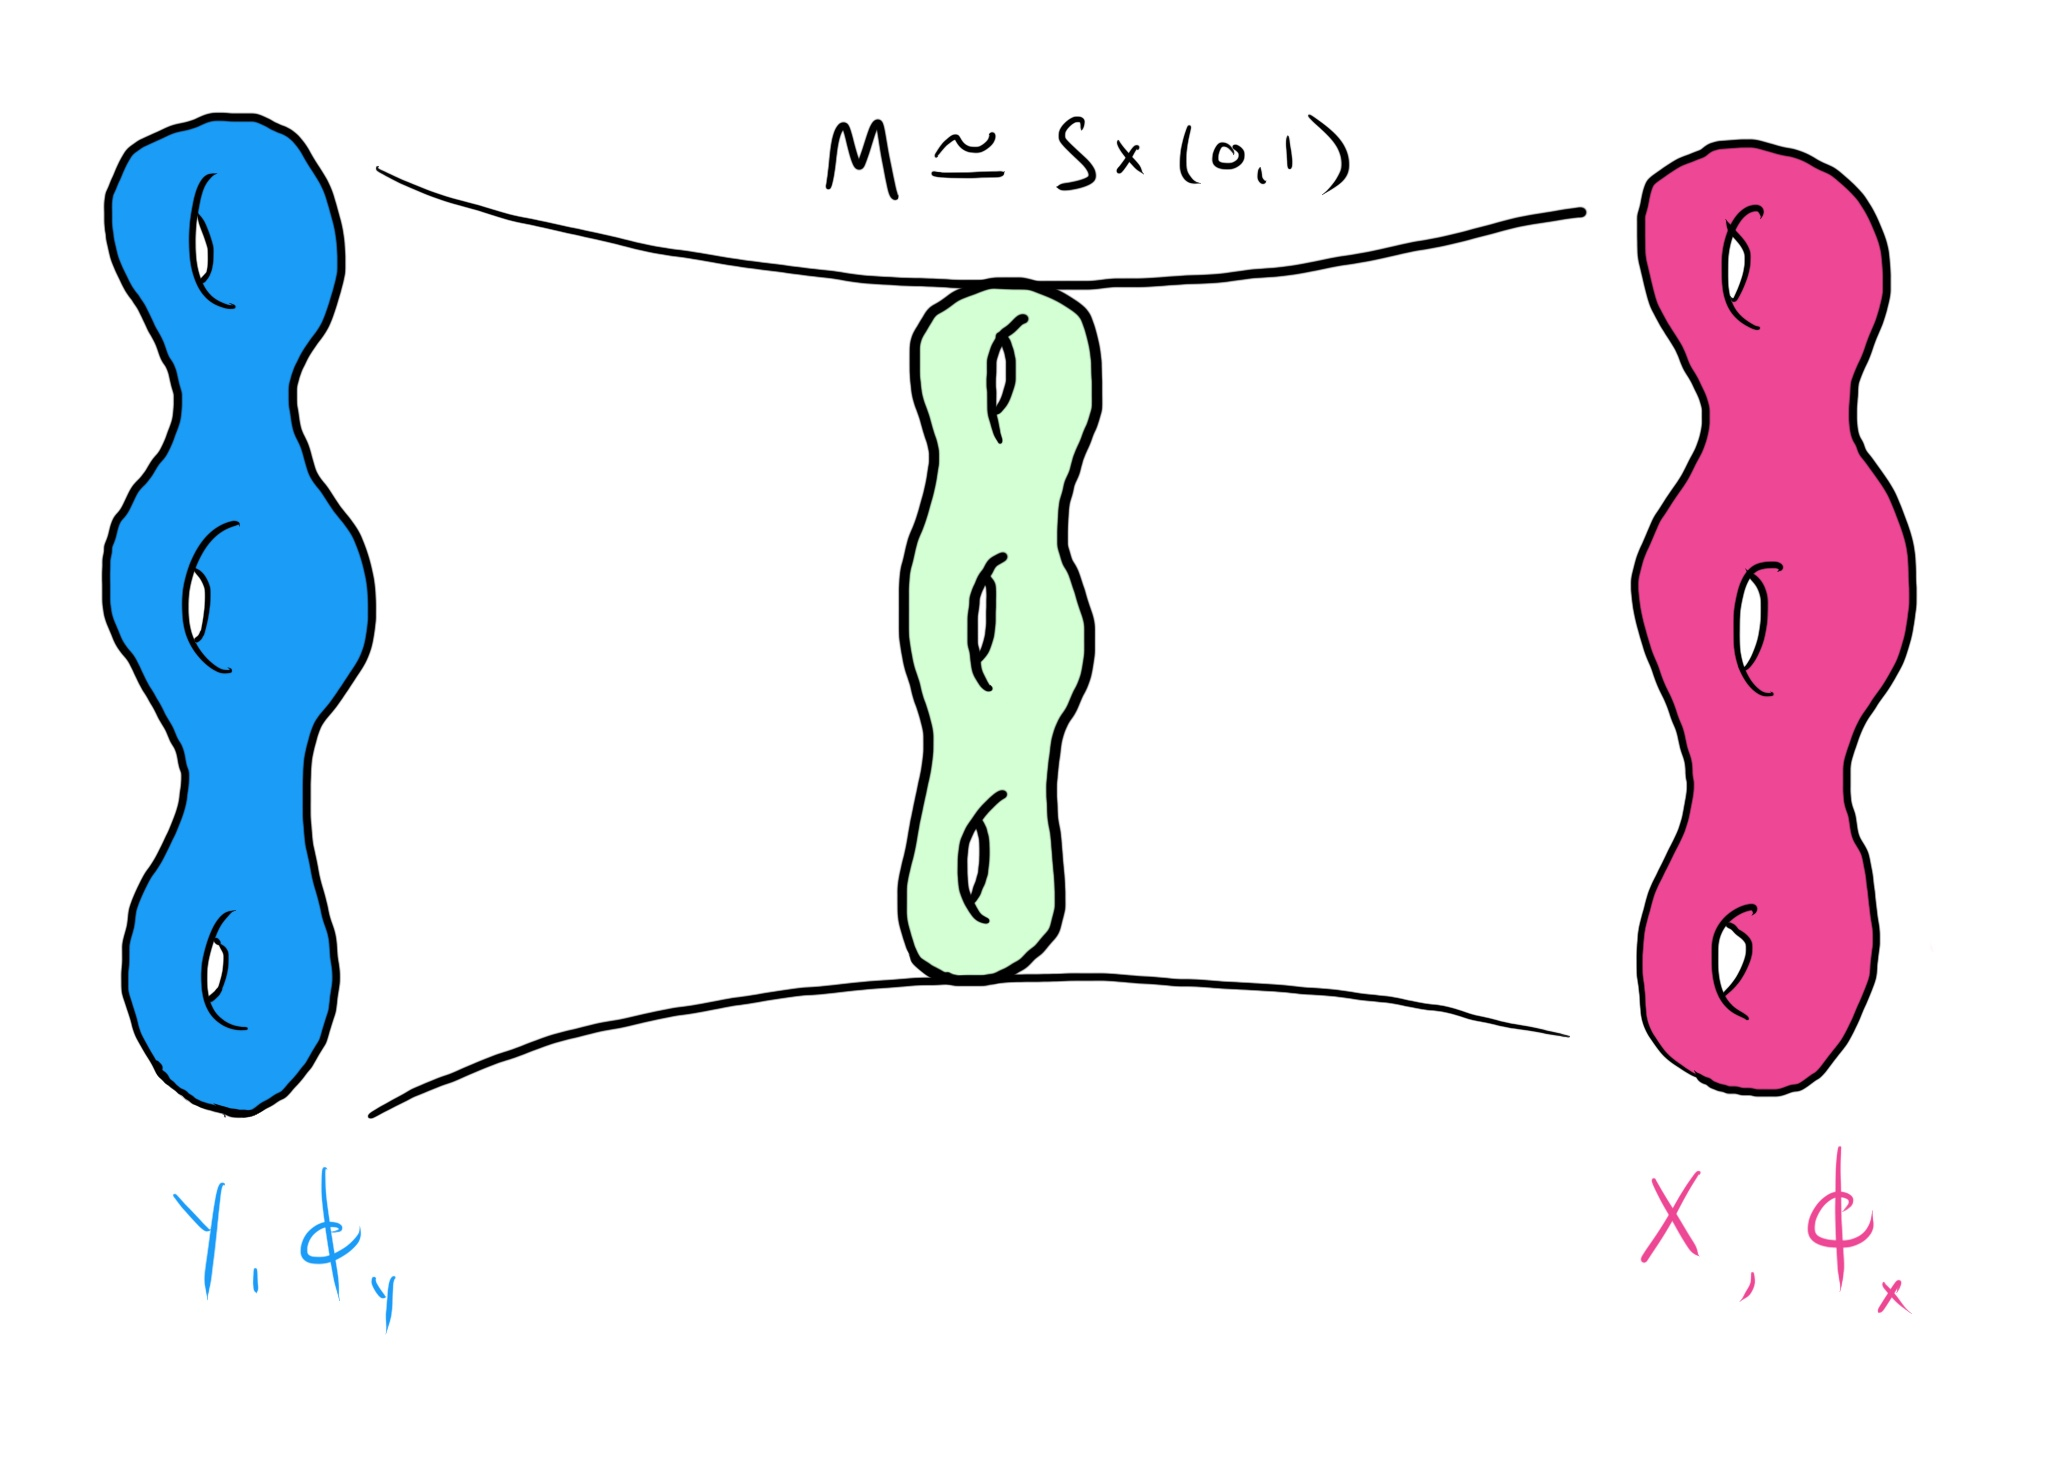
\includegraphics[scale=0.1]{QF-sideways.jpg}


\end{frame}



\begin{frame}{Introduction}
We will consider certain foliations of the ends of $M$ and investigate their limits as the foliations leave the ends. 

\begin{center}
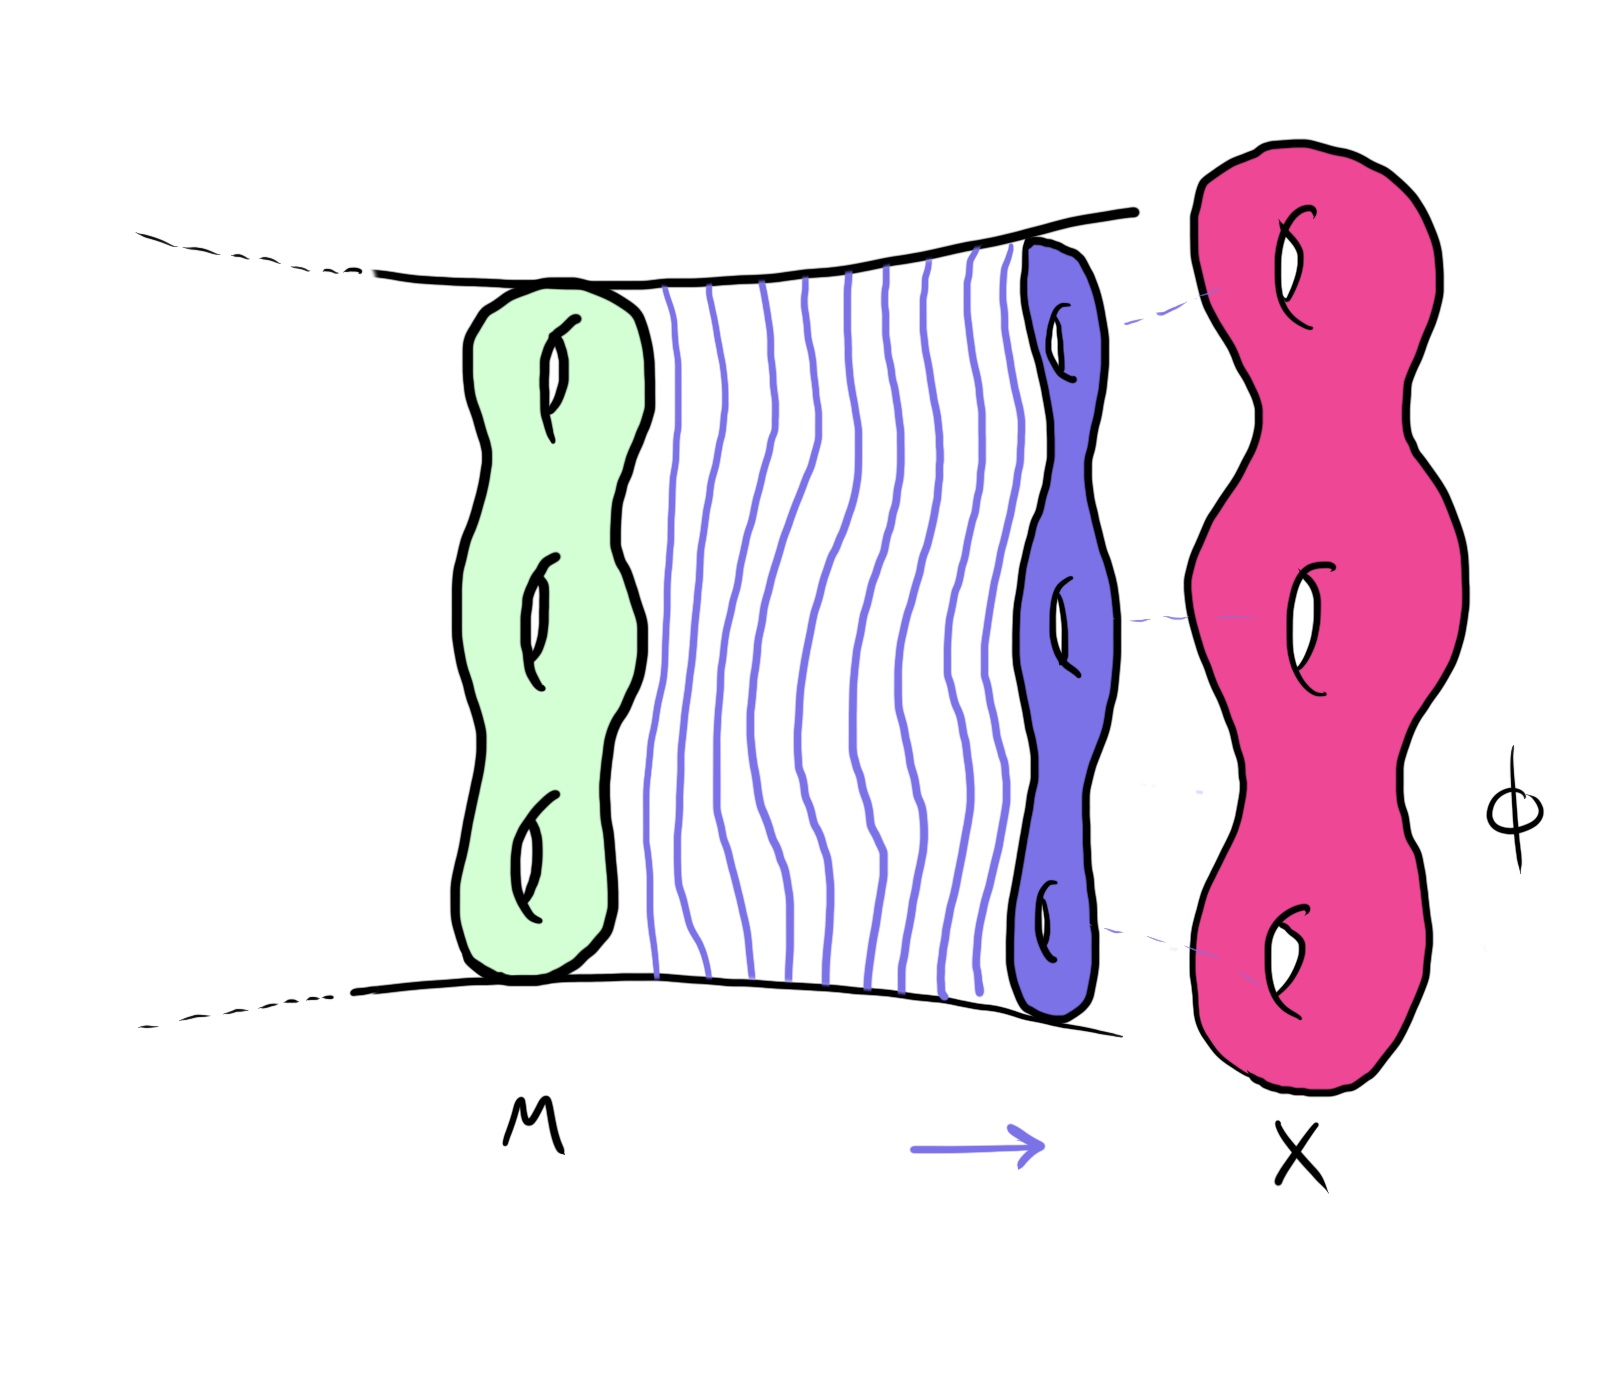
\includegraphics[scale=0.09]{Foliation.jpg}
\end{center}

%Without loss of generality, we will focus on the end of $M$ with surface at infinity $X$ and holomorphic quadratic differential at infinity $\phi$.

We will focus on just one end of $M$. From now on let $X$ denote its surface at infinity and $\phi$ its holomorphic quadratic differential.


\end{frame}


%%%


\begin{frame}{Epstein Surfaces}

C. Epstein describes a way of taking geometric data on the boundary of $\H^3$ and obtaining a surface in $\H^3$.
\newline

\begin{thm}
Let $\Omega$ be a domain in $\CP^1$  and $\sigma$ a $C^k$ conformal metric on $\Omega$, then there exists a unique $C^{k-1}$ map $\mathrm{Ep}_\sigma : \Omega \to \H^3$, called the Epstein map of $\Omega$ for the metric $\sigma$, such that for all $z \in \Omega$,
\[
V_{\mathrm{Ep}_\sigma(z)}(z) = \sigma(z).
\]
Moreover, the image of a point $z$ depends only on the 1-jet of $\sigma$ at $z$.
\label{epstein-map-def} \qed
\end{thm}

\end{frame}


%%%%


\begin{frame}{Epstein Surfaces}


\begin{thm}
Let $\Omega$ be a domain in $\CP^1$  and $\sigma$ a $C^k$ conformal metric on $\Omega$, then there exists a unique $C^{k-1}$ map $\mathrm{Ep}_\sigma : \Omega \to \H^3$, called the Epstein map of $\Omega$ for the metric $\sigma$, such that for all $z \in \Omega$, \ $V_{\mathrm{Ep}_\sigma(z)}(z) = \sigma(z). \qed$
\end{thm}

\begin{center}
\includegraphics<1|handout:0>[scale=0.08]{Epstein-1.jpg}%
\includegraphics<2|handout:0>[scale=0.08]{Epstein-2.jpg}%
\includegraphics<3|handout:0>[scale=0.08]{Epstein-3.jpg}%
\includegraphics<4>[scale=0.08]{Epstein-4.jpg}%
\end{center}

\end{frame}


%


\begin{frame}{Epstein Surfaces}


\begin{thm}
Let $\Omega$ be a domain in $\CP^1$  and $\sigma$ a $C^k$ conformal metric on $\Omega$, then there exists a unique $C^{k-1}$ map $\mathrm{Ep}_\sigma : \Omega \to \H^3$, called the Epstein map of $\Omega$ for the metric $\sigma$, such that for all $z \in \Omega$, \ $V_{\mathrm{Ep}_\sigma(z)}(z) = \sigma(z). \qed$
\end{thm}


\begin{center}
\includegraphics<1|handout:0>[scale=0.08]{Epstein-5.jpg}%
\includegraphics<2|handout:0>[scale=0.08]{Epstein-6.jpg}%
\includegraphics<3|handout:0>[scale=0.08]{Epstein-7.jpg}%
\includegraphics<4|handout:0>[scale=0.08]{Epstein-8.jpg}%
\includegraphics<5|handout:0>[scale=0.08]{Epstein-9.jpg}%
\includegraphics<6|handout:0>[scale=0.08]{Epstein-10.jpg}%
\includegraphics<7|handout:0>[scale=0.08]{Epstein-11.jpg}%
\includegraphics<8>[scale=0.08]{Epstein-12.jpg}%
\end{center}

\end{frame}



%%



\begin{frame}{Properties}

This construction is equivariant with respect to the actions of $\mathrm{SL}_2\C$ on $\CP^1$ and $\H^3$. 

\begin{center}
\includegraphics<2|handout:0>[scale=0.1]{Equivariant-1.jpg}%
\includegraphics<3|handout:0>[scale=0.1]{Equivariant-2.jpg}%
\includegraphics<4|handout:0>[scale=0.1]{Equivariant-3.jpg}%
\includegraphics<5|handout:0>[scale=0.1]{Equivariant-4.jpg}%
\includegraphics<6>[scale=0.1]{Equivariant-5.jpg}%
\end{center}


\end{frame}



%%



\begin{frame}{Properties}

From $\mathrm{Ep}_{N_*\sigma}(N \cdot z) = M \cdot \mathrm{Ep}_{\sigma}(z)$ we get a variant of this Epstein construction for quotients. 
\newline

%\vspace{0.5cm}

In the quasi-Fuchsian case this means if we take a conformal metric $\sigma$ on the surface at infinity $X$, we get an Epstein surface $\mathrm{Ep}_\sigma: X \to M$. (Caution: we say surface even though it may fail to be immersed)

\centering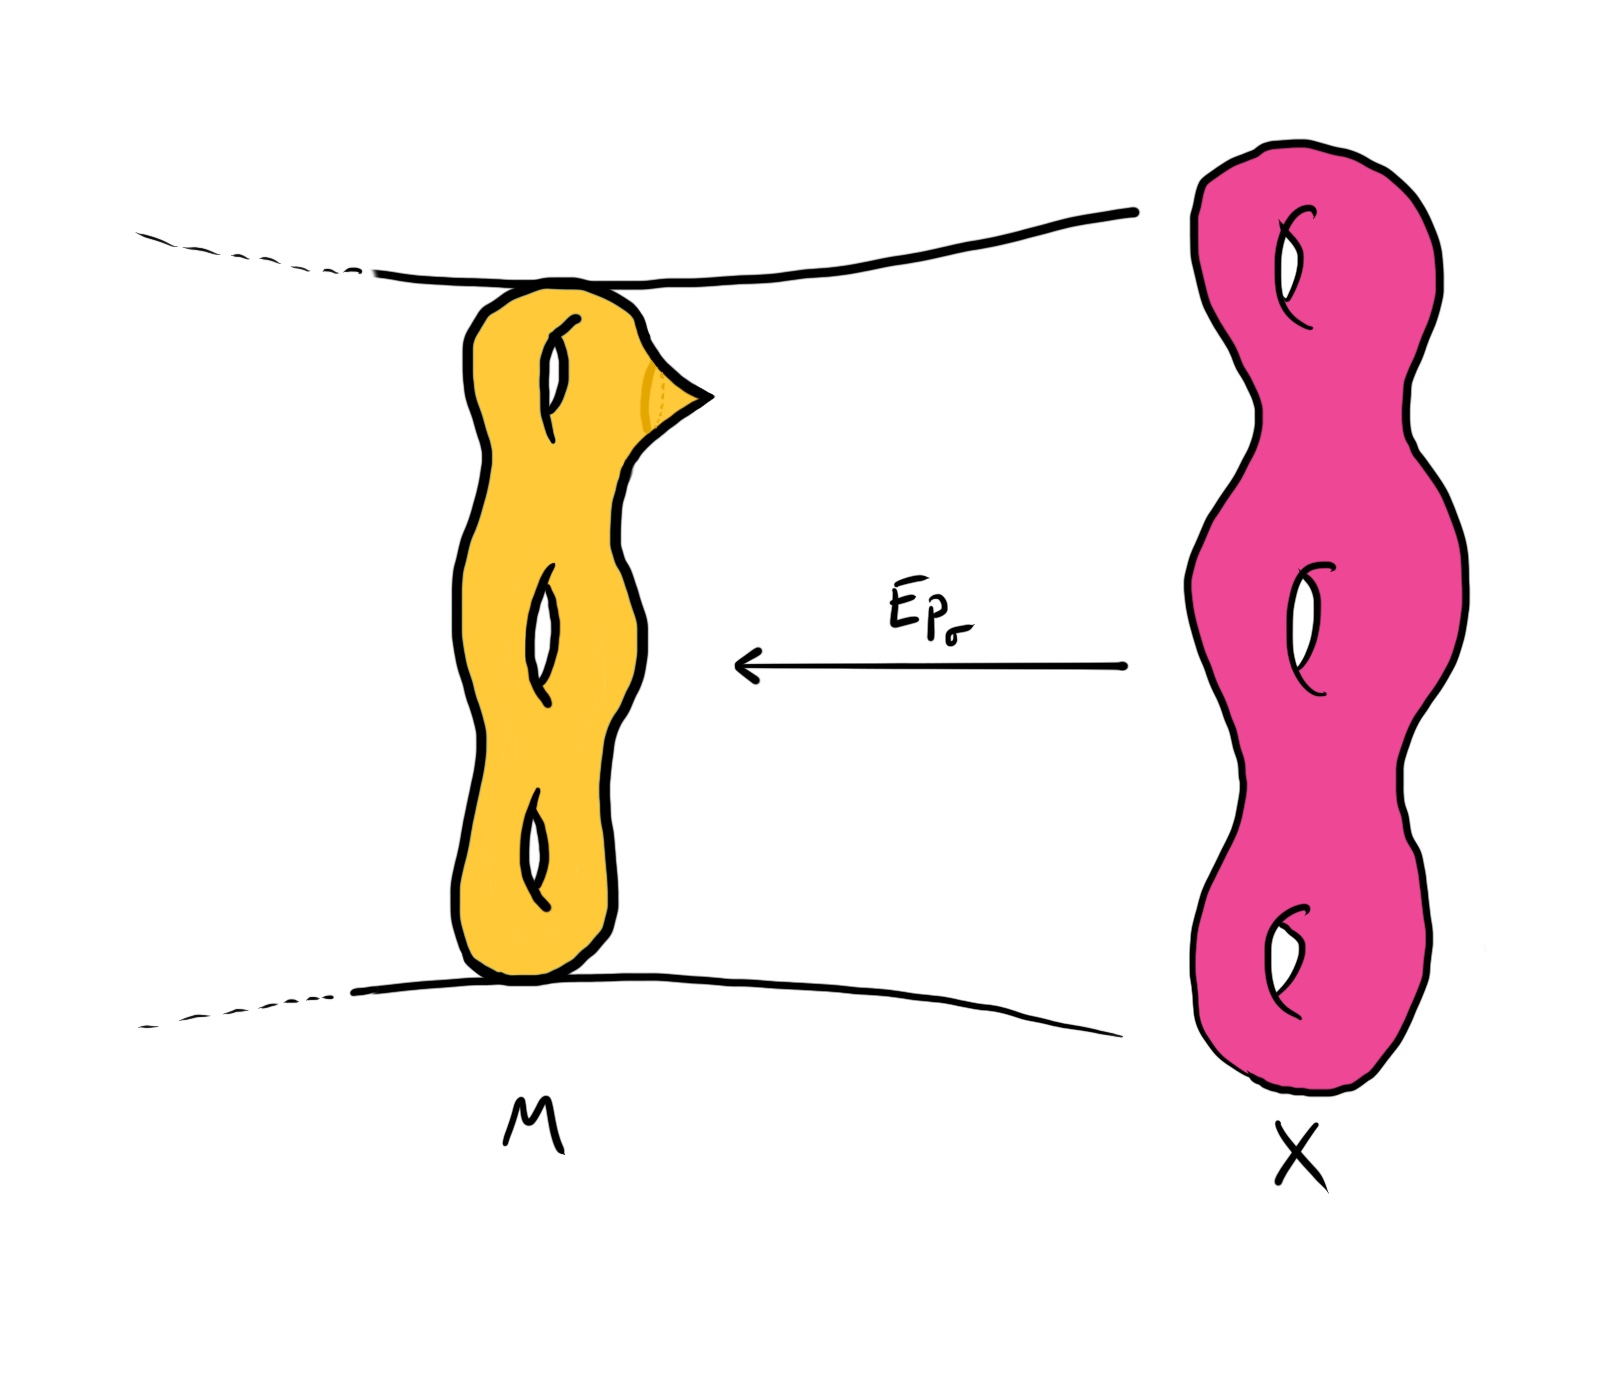
\includegraphics[scale=0.11]{Quotients.jpg}

\end{frame}


%%


\begin{frame}{Properties}

The Epstein construction behaves well under a normal flow. 

Flowing $\mathrm{Ep}_\sigma$ for time $t$ in the normal direction gives a parallel copy of the Epstein surface at distance $t$ from the original copy. This parallel surface is also obtained as the Epstein surface $\mathrm{Ep}_{e^{2t}\sigma}$.

\vspace{-0.2cm}

\begin{center}
\includegraphics<1|handout:0>[scale=0.09]{Parallel-1.jpg}%
\includegraphics<2|handout:0>[scale=0.09]{Parallel-2.jpg}%
\includegraphics<3|handout:0>[scale=0.09]{Parallel-3.jpg}%
\includegraphics<4|handout:0>[scale=0.09]{Parallel-4.jpg}%
\includegraphics<5|handout:0>[scale=0.09]{Parallel-5.jpg}%
\includegraphics<6|handout:0>[scale=0.09]{Parallel-6.jpg}%
\includegraphics<7|handout:0>[scale=0.09]{Parallel-7.jpg}%
\includegraphics<8|handout:0>[scale=0.09]{Parallel-8.jpg}%
\includegraphics<9|handout:0>[scale=0.09]{Parallel-9.jpg}%
\includegraphics<10|handout:0>[scale=0.09]{Parallel-10.jpg}%
\includegraphics<11>[scale=0.09]{Parallel-11.jpg}%
\end{center}

\end{frame}


%%


\begin{frame}{The Poincar\'e Family}



We call the unique hyperbolic conformal metric $h$ on $X$ the Poincar\'e metric and its Epstein surface $\mathrm{Ep}_h: X \to M$ the Poincar\'e surface of $X$. 
\newline \pause

The family obtained by parallel flowing $\mathrm{Ep}_h$ we call the Poincar\'e Family, and this family is given as $(\mathrm{Ep}_{e^{2t}h})_{t\geq 0}$.
\newline \pause

For $t > c = c(\phi, h)$ the surfaces $\mathrm{Ep}_{e^{2t}h}$ are embedded, and so for $t$ sufficiently large, this family forms a foliation of the end of $M$.
\newline \pause

Notice that after rescaling by $\epsilon = e^{-2t}$, the conformal metrics $\rho_\epsilon$ of Poincar\'e family satisfies $\epsilon \rho_\epsilon \to h$ as $\epsilon \to 0$.


\end{frame}


%%


\begin{frame}{Asymptotically Poincar\'e Families}

\begin{defn}
\label{asym-def}
Let $S_\epsilon$ for $\epsilon \in (0,1)$ be a family of embedded Epstein surfaces for the conformal metrics $\sigma(\epsilon)$. 
We call this family \emph{asymptotically Poincar\'e} if \pause
\begin{enumerate}
    \item there exists a scaling function $f:[0,1) \to [0,\infty)$ so that the path
    \[
f\sigma:(0,1) \to \mathrm{Met}^\infty(X)
\]
is differentiable and converges to the Poincar\'e metric on $X$ as $\epsilon \to 0$, \pause
    \item the function $f$ is smooth and has simple zero at 0, and \pause
    \item the continuous extension $\gamma:[0,1) \to \mathrm{Met}^\infty(X)$ of $f \sigma$ is differentiable.
\end{enumerate}

\end{defn}

\end{frame}


%%


\begin{frame}{Asymptotically Poincar\'e Families Foliate}

\begin{prop*}[Q.]
Let $S_\epsilon$ be an asymptotically Poincar\'e family for the conformal metrics $\sigma(\epsilon)$. There exists a $\delta > 0$ (depending on the family) such that for $\epsilon \in (0,\delta)$ the surfaces $S_\epsilon$ foliate the end of $M$.
\end{prop*} \pause

\begin{proof}

\begin{itemize}

\item The 1-parameter family of associated Epstein maps gives a map $\mathrm{Ep}_{\sigma}: [0,1) \times X \to M \sqcup X$ that restricts to the identity on the boundary $\{ 0 \} \times X \to X$. \pause

\item The function given by $E(\epsilon,x) = \mathrm{Ep}_\sigma(\epsilon^2,x)$ has invertible derivative on the boundary and so it is a local $C^1$-diffeomorphism from a neighborhood of the boundary into $M \sqcup X$. \pause

\item Therefore, the restriction of $E$ to $[0, \delta^2) \times X$, for some small
enough $\delta$, is a diffeomorphism onto a collar neighborhood of $X$ in $M \sqcup X$.

\end{itemize}

\end{proof}

\end{frame}


%


\begin{frame}{Main Results}

\begin{thm*}[Q.]
Let $S_\epsilon$ for $\epsilon \in (0,1)$ be an asymptotically Poincar\'e family of surfaces for the conformal metrics $\sigma(\epsilon)$. 
If $h$ is the Poincar\'e metric of $X$ and $\phi$  the holomorphic quadratic differential at infinity, then in Teichm\"uller space $\mathcal{T}(X)$ we have 
\[
[I(\sigma(\epsilon))] \to [h]
\quad \text{ and } \quad
[\two(\sigma(\epsilon))] \to [h]
\quad \text{ as } \epsilon \to 0.
\]
Moreover, the tangent vectors at $\epsilon = 0$ in $T_{[h]} \mathcal{T}(X)$ are given by 
\[
\dot{[I(\sigma(\epsilon))]}  = 4 f'(0) \mathrm{Re}(\phi) \quad \text{ and } \quad \dot{[\two(\sigma(\epsilon))]} = 0.
\]
\end{thm*}

\end{frame}


%%


\begin{frame}{Riemannian Model of $\mathcal{T}(X)$}

We model $\mathcal{T}(X)$ as the quotient $\mathrm{Met}^\infty(X)/(\mathrm{Diff}_0^\infty(X) \ltimes P^\infty(X))$ but we will first work with Sobolev tensors. 
\newline

Denote by $\mathrm{Met}^s(X)$ the set of Riemannian metrics of Sobolev class $H^s$ for a fixed $s > 3$ and note that $\mathrm{Met}^\infty(X) = \cap_{s > 3} \mathrm{Met}^s(X)$
\newline

With these regularity assumptions $T_h\mathrm{Met}^s(X)$ is a Hilbert space.



\end{frame}


%%


\begin{frame}{Riemannian Model of $\mathcal{T}(X)$}
$T_h\mathrm{Met}^s(X)$ decomposes as the orthogonal direct sum 
\[
\{ g \ | \ \mathrm{tr}_h (g) = 0 = \mathrm{div}_h(g) \} \oplus \{\mathcal{L}_V h + u h \ |\ u \in H^s \text{, } V \in \Gamma(TX) \}.
\] \pause 

\begin{center}
\includegraphics<1|handout:0>[scale=0.09]{Tangent-1.jpg}%
\includegraphics<2|handout:0>[scale=0.09]{Tangent-2.jpg}%
\includegraphics<3|handout:0>[scale=0.09]{Tangent-3.jpg}%
\includegraphics<4|handout:0>[scale=0.09]{Tangent-4.jpg}%
\includegraphics<5>[scale=0.09]{Tangent-5.jpg}%
\end{center}

\end{frame}


%%


\begin{frame}{Riemannian Model of $\mathcal{T}(X)$}
The set $\{ g \ | \ \mathrm{tr}_h (g) = 0 = \mathrm{div}_h(g) \}$ is a model for the tangent space to the quotient at $[h]$. 
\newline

This is true for any $s$, and each such $g$ is a smooth tensor. So this set is identified with the tangent space to Teichm\"uller space.
\begin{align*}
T_{[h]}\mathcal{T}(X)
&= \{ g \ | \ \mathrm{tr}_h (g) = 0 = \mathrm{div}_h(g) \} \\
&= \{ \mathrm{Re}(\psi) \ | \ \psi \text{ a holomorphic quadratic differential on } X \}.
\end{align*} \pause

The projection $\mathrm{Met}^\infty(X) \to \mathcal{T}(X)$ is continuous and its derivative at $h$ is given by orthogonal projection onto $\{ \mathrm{Re}(\psi) \}$




\end{frame}







\begin{frame}{Proof}
Returning to our theorem, we are given that $\gamma:[0,1) \to \mathrm{Met}^\infty(X)$ is continuous and differentiable at $\epsilon = 0$. 
Therefore, we also have that $\gamma$ is continuous to $\mathrm{Met}^s(X)$, for each $s$, and is differentiable at $\epsilon = 0$. \pause
\newline

In $\mathrm{Met}^s(X)$ we can write 
\[
I(\sigma(\epsilon)) =  \frac{1}{4\epsilon f'(0)} h + \frac{1}{4 f'(0)} \dot{\gamma} + \frac{1}{2} h + \mathrm{Re}(\phi) + O(\epsilon), \pause
\]
so that 
\[
I_\epsilon := 4\epsilon f'(0)I(\sigma(\epsilon)) = h + \epsilon( \ \dot{\gamma} + 2 f'(0)h + 4 f'(0) \mathrm{Re}(\phi) \ ) + O(\epsilon^2).
\]

\end{frame}


%%


\begin{frame}{Proof}
From the expression
\[
I_\epsilon = h + \epsilon( \ \dot{\gamma} + 2 f'(0)h + 4 f'(0) \mathrm{Re}(\phi) \ ) + O(\epsilon^2)
\]
we can see that $I_\epsilon \to h$ in $\mathrm{Met}^s(X)$ for all $s$, implying $I_\epsilon \to h$ in $\mathrm{Met}^\infty(X)$. 
\newline

Moreover, the derivative at $\epsilon = 0$ is 
\[
\dot{I_\epsilon}  = \dot{\gamma} + 2 f'(0) h + 4 f'(0) \mathrm{Re}(\phi).
\]

\end{frame}


%%


\begin{frame}{Proof}

\begin{center}
\includegraphics<1|handout:0>[scale=0.09]{Teich-1.jpg}%
\includegraphics<2|handout:0>[scale=0.09]{Teich-2.jpg}%
\includegraphics<3|handout:0>[scale=0.09]{Teich-3.jpg}%
\includegraphics<4|handout:0>[scale=0.09]{Teich-4.jpg}%
\includegraphics<5>[scale=0.09]{Teich-5.jpg}%
\end{center}

\end{frame}


%%


\begin{frame}


Therefore, as $I_\epsilon \to h$ in $\mathrm{Met}^\infty(X)$ we have that $[I(\sigma(\epsilon))] = [I_\epsilon] \to [h]$ in $\mathcal{T}(X)$. \pause

\vspace{0.5cm}
 
And since
\[
\dot{I_\epsilon}  = \dot{\gamma} + 2 f'(0) h + 4 f'(0) \mathrm{Re}(\phi), 
\]
we see
\[
\dot{[I(\sigma(\epsilon))]} = 4f'(0)\mathrm{Re}(\phi).
\] \pause

The same arguments work for $\two(\sigma(\epsilon))$. \qed

\end{frame}


%%


\begin{frame}{Applications}
We apply this result to two foliations by constant curvature surfaces.
\newline \pause
	
	\begin{thm*}[Labourie, 1991 - 1992]
Let $E$ be an end of a quasi-Fuchsian manifold $M$, then for each $k \in (-1,0)$, there exists a unique (incompressible) surface embedded in $E$ with constant Gaussian curvature $k$. Moreover, this family of surfaces foliates the end $E$.
\end{thm*}\pause

\vspace{0.5cm}

\begin{thm*}[Mazzeo-Pacard, 2011]
Each end of a quasi-Fuchsian manifold admits a unique foliation by constant mean curvature surfaces. 
\end{thm*}

	
\end{frame}


%%


\begin{frame}{A Conjecture of Labourie}
Labourie called the constant Gaussian surfaces $k$-surfaces and he discusses how their first and second fundamental forms may be considered as paths in Teichm\"uller space.

\begin{center}
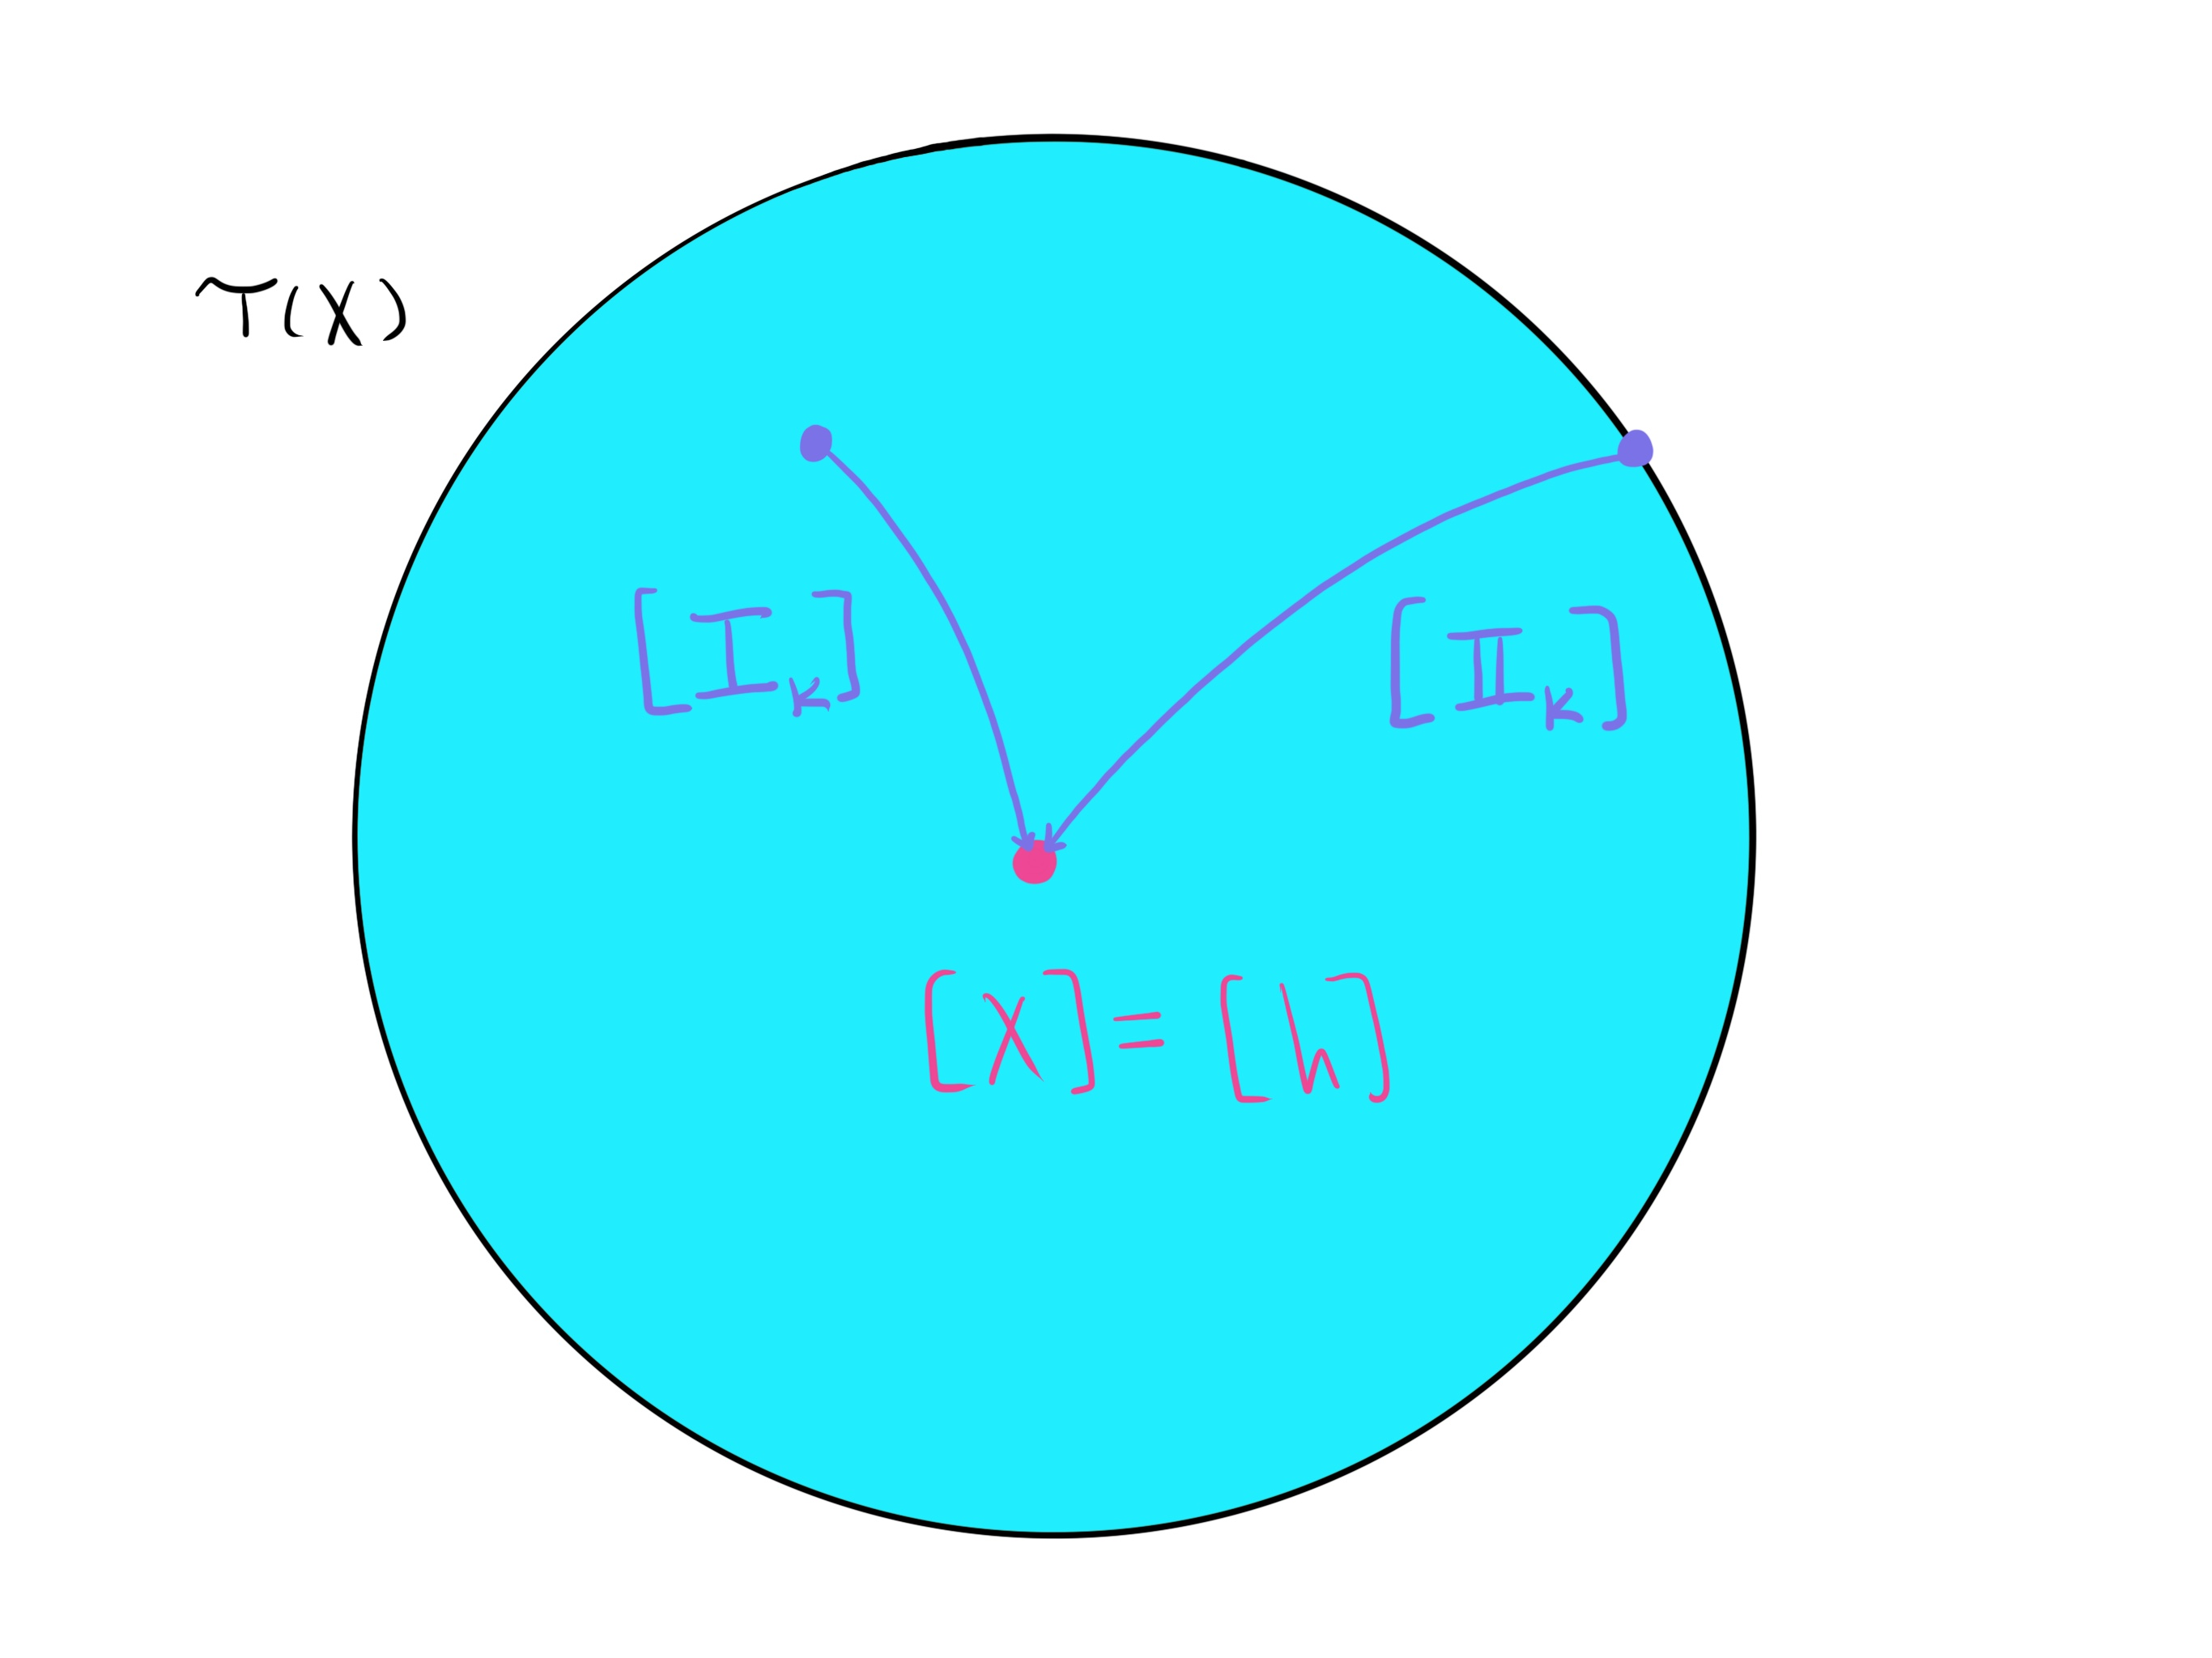
\includegraphics[scale=0.07]{Teich-paths-1.jpg}
\end{center}


\end{frame}


%%


\begin{frame}{A Conjecture of Labourie}

\vspace{-0.5cm}
\begin{center}
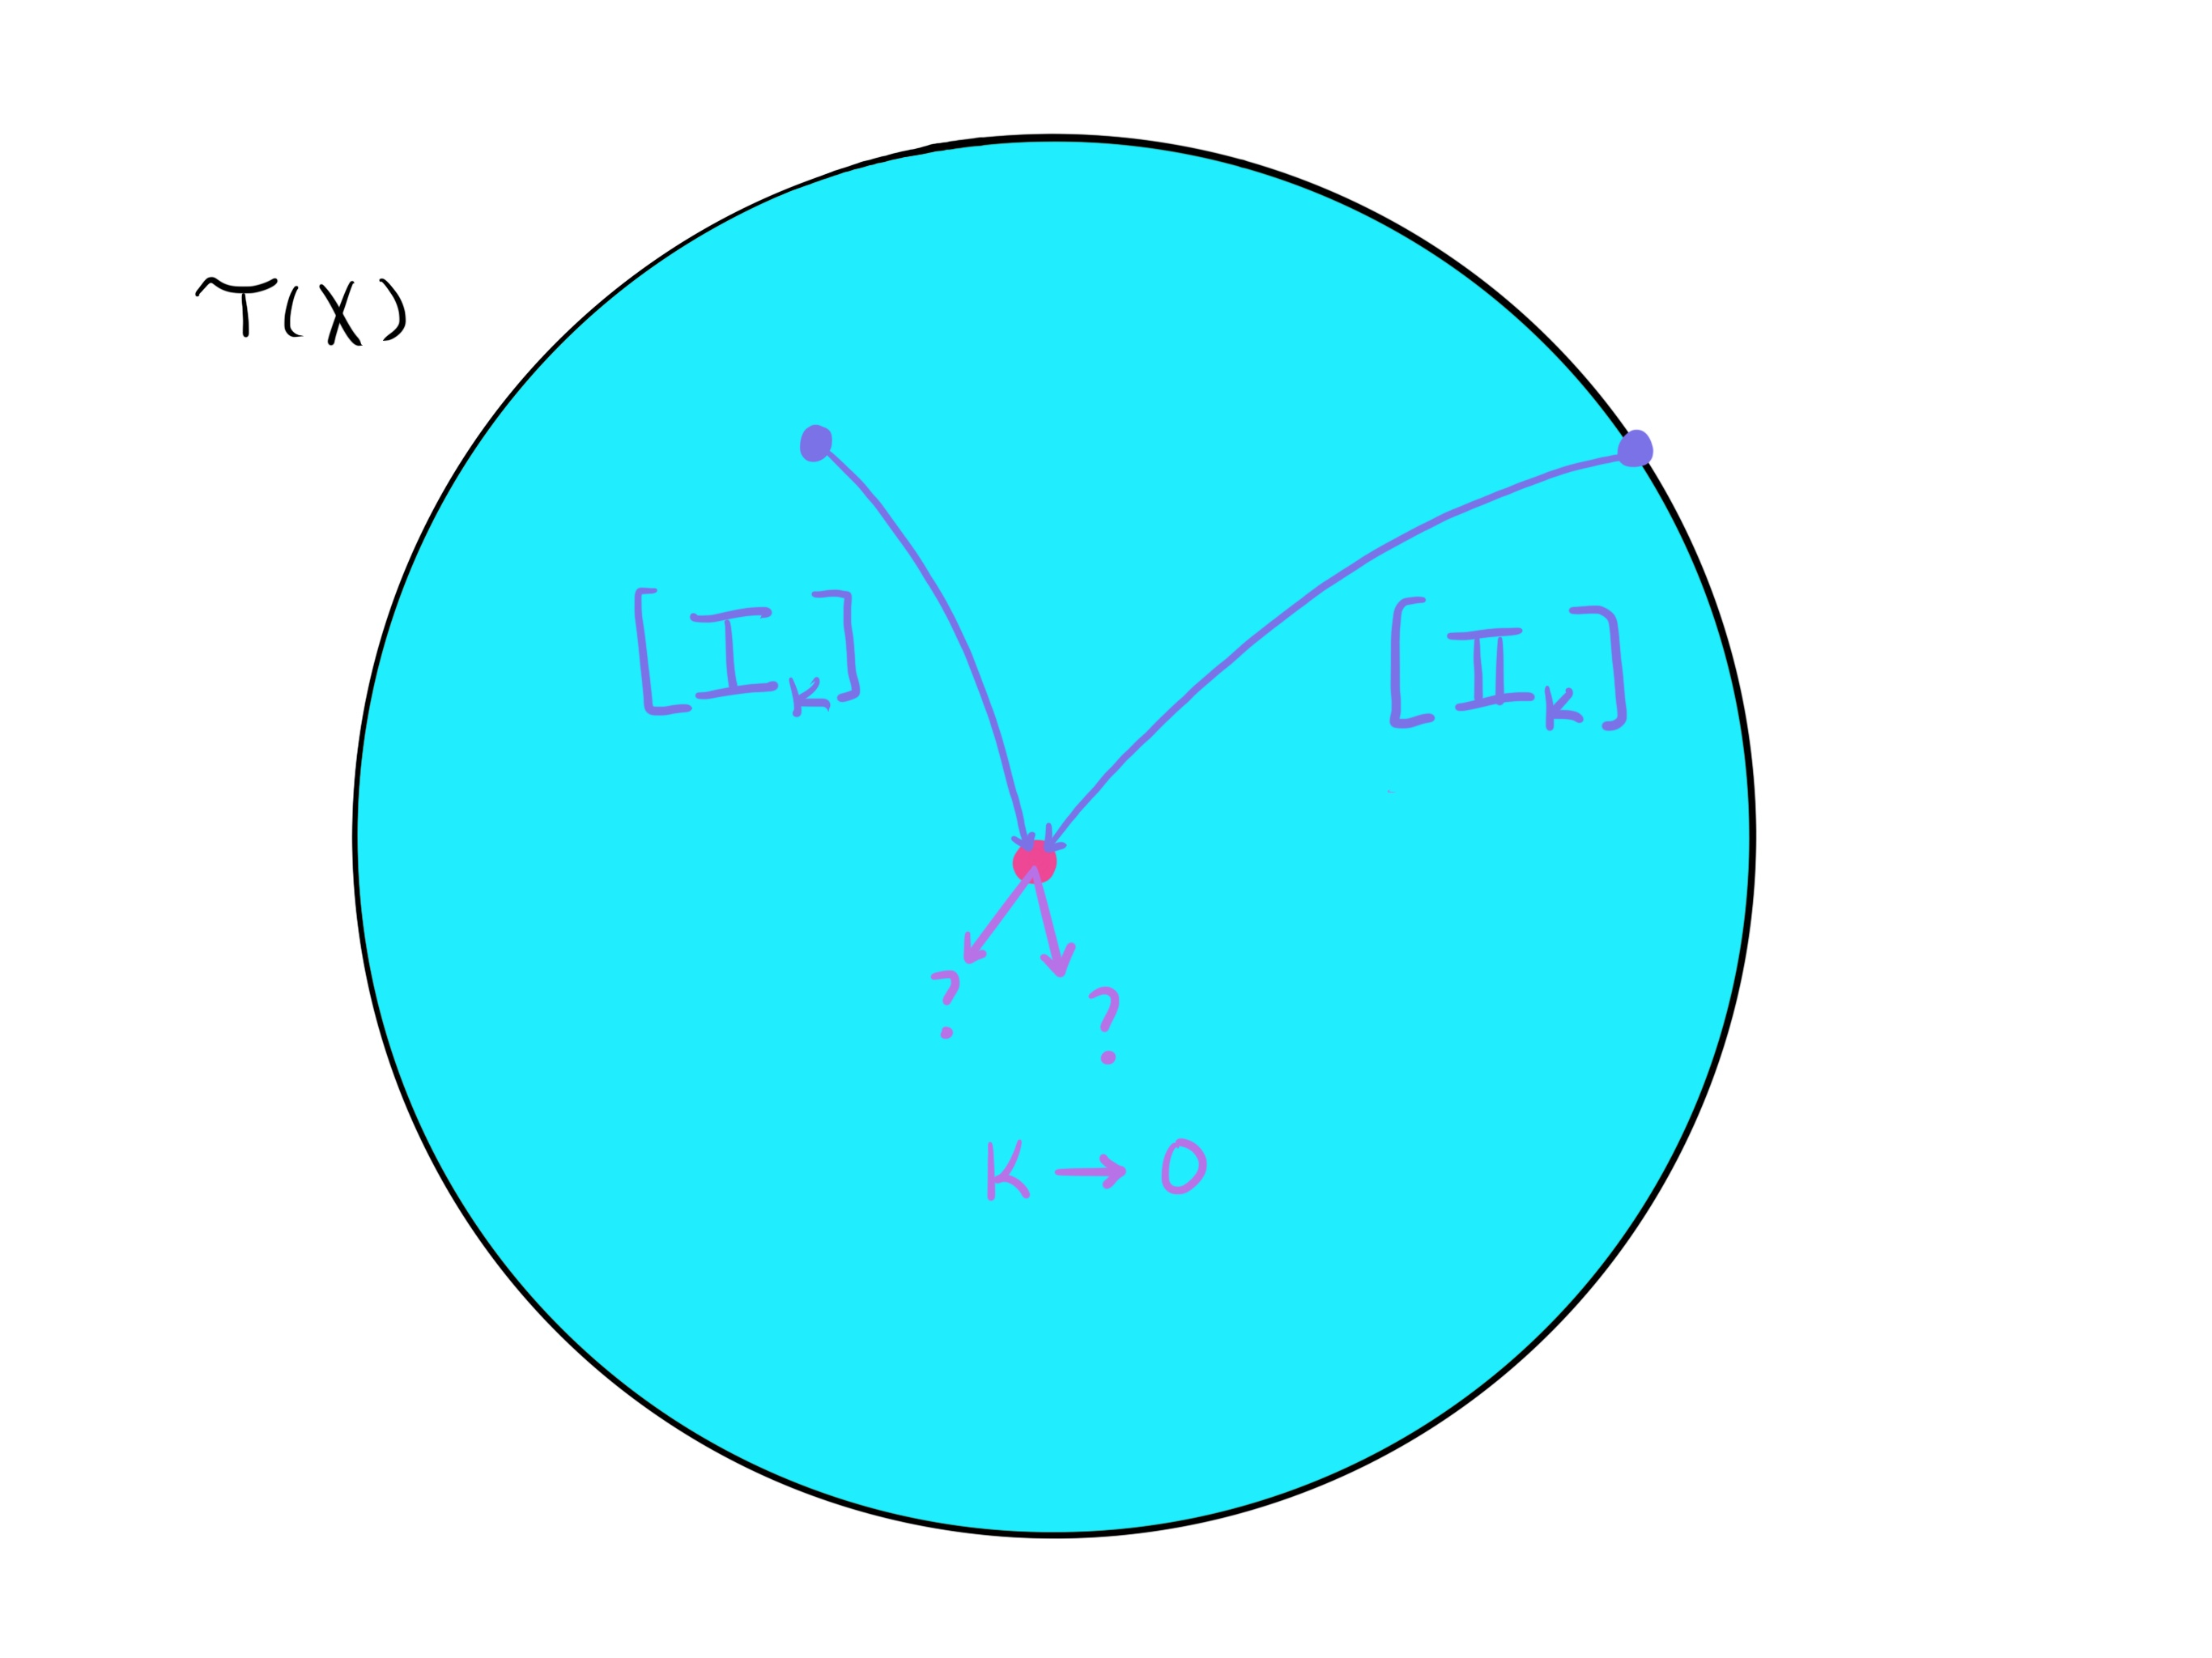
\includegraphics[scale=0.07]{Teich-paths-2.jpg}
\end{center}

\vspace{-0.5cm}
He shows that as $k \to 0$, the paths $[I_k]$ and $[\two_k]$ converge to $[X] = [h]$ and he asks after the tangent vectors to these paths at $k=0$. 
\newline

He conjectures $\dot{[I_k]}$ is related to the holomorphic quadratic differential $\phi$.
\end{frame}


\begin{frame}{A Conjecture of Labourie}
 
\begin{thm}[Q.] \label{labourie-conjecture-proof}
Let $I_k$ and $\two_k$ be the first and second fundamental forms of the family of $k$-surfaces in an end of a quasi-Fuchsian manifold. 
Let $\phi$ be the holomorphic quadratic differential at infinity of $M$. 
Then, as $k \to 0$, the tangent vectors to $[I_k]$ and $[\two_k]$ in Teichm\"uller space are given by 
\[
\dot{[I_k]} = - \mathrm{Re}(\phi) \quad \text{and } \quad   \dot{[\two_k]} = 0.
\]
\end{thm} \pause

\vspace{0.5cm}

We prove this by presenting the $k$-surfaces as Epstein surfaces (for $k$ near 0) and showing they form an asymptotically Poincar\'e family.
\newline

This also gives another proof of the existence of $k$-surfaces, for $k$ near 0.

\end{frame}


%%


\begin{frame}{Proof}
To present a $k$-surface as an Epstein surface we must find a conformal metric $\sigma$ so that
\[
K(I(\sigma)) = \frac{4K(\sigma)}{(1-K(\sigma))^2 - 16|B(\sigma)|^2\sigma^{-2}} = k.
\] \pause

We focus on solving 
\begin{equation}\tag{$\ast$}\label{k-surface-eqn}
4K(\sigma) = k \left((1-K(\sigma))^2 - 16|B(\sigma)|^2\sigma^{-2} \right)
\end{equation}
as for small $k$ this suffices. 
\newline \pause


Notice though, that when $k=0$ this reads $K(\sigma) = 0$, which has no solutions on $X$.
\end{frame}


%%


\begin{frame}{Proof}
Our technique is to use the Implicit Function Theorem to obtain solution for each $k$ near 0. But since there are no solutions for $k = 0$ we rescale the equation by considering the function $f(k) = \frac{1-\sqrt{1+k}}{1+\sqrt{1+k}}$. 
\newline \pause

If $\sigma$ solves \eqref{k-surface-eqn} then $\tau = f(k)\sigma$ solves 
\begin{multline*}
(2+k)(1+K(\tau))^2  \\ + 2\sqrt{1+k}\left(1-K(\tau)^2 \right) +16\left(2\sqrt{1+k} - 2 - k  \right)\frac{|B(\tau)|^2}{\tau^2} = 0
\end{multline*}or 
\[
F(k,\tau) = 0.
\]\pause


Notice that $F(0,\tau) = 0$ is equivalent to $K(\tau) = -1$, which has the solution $\tau = h$. 
\end{frame}


%%


\begin{frame}{Proof}
Since we have a solution for $k = 0$, we can then use the Implicit Function Theorem to get solution for $k$ near zero as well. 
\newline

The function $F$ extends from the smooth setting to one of $(-1,0) \times \mathrm{Conf}^s(X) \to H^{s-2}(X)$. \pause
\newline

We compute
\[
DF_{(0,h)}(\dot{k},\dot{\tau}) = 4D K_h(\dot{\tau}) =-2(\Delta_h - Id)\frac{\dot{\tau}}{h}
\]
and see that $D_2F_{(0,h)} = 4D K_h: H^s(X) \to H^{s-2}(X)$ is an isomorphism.
\newline

\end{frame}


%%

\begin{frame}{Proof}
Consequently, there exists a neighborhood $V$ of $0$ and a curve $\gamma : V \to \mathrm{Conf}^s(X)$ with $\gamma(0) = h$ and $F(k, \gamma(k)) = 0$. 
%Moreover, these are the only solutions to $F(k,\tau) = 0$ in $V$, and $\gamma$ is smooth since $F$ is smooth.
\newline \pause

Elliptic regularity theory applied to $D K_h$ tells us that there is a $\delta >0$ such that 

\begin{itemize}

	\item $\gamma(k)$ is a smooth conformal metric for each $k \in (-\delta,\delta)$, \pause
	
	\item the path $\gamma: (-\delta,\delta) \to \mathrm{Conf}^\infty(X)$ is a smooth path. \pause
	
\end{itemize}
\vspace{0.5cm}

To complete the proof we take $\sigma(k) := f(k)^{-1}\gamma(k)$ for $k \in (-\delta,0)$.
\newline

The family of Epstein surfaces for $\sigma(k)$ then satisfy the definition of an asymptotically Poincar\'e family and our main theorem applies.  \qed
\end{frame}


%%


\begin{frame}{Constant Mean Curvature Surfaces}

\begin{thm*}[Mazzeo-Pacard, 2011]
The ends of a quasi-Fuchsian manifold admit unique foliations by constant mean curvature surfaces. 
\end{thm*}
\vspace{0.5cm}

\begin{thm*}[Q.]
Let $I_k$ and $\two_k$ be the first and second fundamental forms of the Epstein surface with constant mean curvature $-\sqrt{1+k}$.
Let $\phi$ be the holomorphic quadratic differential at infinity. 
Then, as $k \to 0$, the tangent vectors to $[I_k]$ and $[\two_k]$ in Teichm\"uller space are given by 
\[
  \dot{[I_k]}= - \mathrm{Re}(\phi) \quad \text{and } \quad \dot{[\two_k]} = 0.
\]
\end{thm*}

\end{frame}


%%


\begin{frame}{Proof}
The proof proceeds the same as in the constant Gaussian curvature case. However, here we wish to solve the equation 
\[
H(\mathrm{Ep}_\sigma)
= \frac{K(\sigma)^2 - 1 - 16|B(g_{\CP^1},\sigma)|^2\sigma^{-2}}{(K(\sigma) - 1)^2 - 16|B(g_{\CP^1},\sigma)|^2\sigma^{-2}} = -\sqrt{1 + k}.
\]\pause

Using the same scaling function $f(k)$ we are led to consider solutions to a function $G(k,\tau) = 0$, which has partial derivative $D_2G_{(0,h)} = 2D K_h(\dot{\tau})$. 
\newline \pause

%\[
%G(k,\tau) = 1+\sqrt{1+k} + 2\sqrt{1+k}K(\tau) + (-1 + \sqrt{1+k})(K(\tau)^2 - \frac{16}{\tau^2}|B(\tau)|^2).
%\]
%And search for solutions to $G(k,\tau) = 0$. Again we have $\tau = h$ solves $G(0,\tau) = 0$.

The Implicit Function Theorem then gives solutions for $k$ near zero. \qed

\end{frame}


%%


%\begin{frame}{Proof}
%And so we again use the Implicit Function Theorem to get solutions for $k$ near 0 by computing 
%\[
%dG_{(0,h))}(\dot{k},\dot{\tau}) = -4 \frac{|\phi|^2}{h^2} \dot{k} + 2 D K_h(\dot{\tau}).
%\]
%We have $D_2G_{(0,h)} = 2D K_h(\dot{\tau})$, which is an isomorphism. The proof the proceeds identically to the $k$-surface case. \qed
%\end{frame}


%%


\begin{frame}
\begin{center}
Thank you!
\end{center}
\end{frame}










\end{document}